\documentclass[11pt,a4paper]{article}

% Essential packages
\usepackage[utf8]{inputenc}
\usepackage[T1]{fontenc}
\usepackage{geometry}
\usepackage{xcolor}
\usepackage{tikz}
\usepackage{fontawesome}
\usepackage{microtype}
\usepackage{graphicx}
\usepackage{titlesec}
\usepackage{etoolbox}
\usepackage{lmodern}  % Better font

\usepackage{settings}



% Define a sophisticated and harmonious color palette
\definecolor{primaryAccent}{HTML}{3D5A80}      % Cool Blue
\definecolor{secondaryAccent}{HTML}{E07A5F}    % Terracotta
\definecolor{tertiaryAccent}{HTML}{81B29A}     % Sage Green
\definecolor{quaternaryAccent}{HTML}{F4A261}   % Sandy Orange
\definecolor{darkShade}{HTML}{293241}          % Dark Slate Blue
\definecolor{lightShade}{HTML}{F8F9FA}         % Very Light Grey (instead of Cream for cleaner look)

% Gradient stops for side bar using the new palette
\definecolor{accentGradient1}{HTML}{3D5A80}    % Cool Blue
\definecolor{accentGradient2}{HTML}{5A7D9A}    % Lighter Cool Blue
\definecolor{accentGradient3}{HTML}{81B29A}    % Sage Green

% Update accent line color (if used, otherwise can be removed)
\definecolor{SwishLineColour}{HTML}{81B29A}  % Sage Green

% Set minimal margins
\geometry{left=2.5cm, right=2.5cm, top=2.5cm, bottom=2.5cm, heightrounded}


% Custom formatting
\setlength{\parindent}{0pt}
\setlength{\parskip}{1.0em}
\pagestyle{empty}
\titlespacing*{\section}{0pt}{1.5ex plus 1ex minus .2ex}{1.0ex plus .2ex}

% Title section formatting
\titleformat{\section}{\normalfont\large\bfseries}{}{0em}{\color{primaryAccent}} % Use Cool Blue for section titles

% Add subtle highlight to important paragraphs
\newcommand{\highlightpara}[1]{%
  \begin{adjustwidth}{0.5cm}{0.5cm}
    \begingroup
    \setlength{\parskip}{0.5em}
    \color{darkShade}
    #1
    \endgroup
  \end{adjustwidth}
}

% Create a subtle separator that can be used between sections
\newcommand{\elegantseparator}{%
  \begin{center}
    \begin{tikzpicture}
      \draw[primaryAccent!40, line width=0.4pt] (0,0) -- (3,0);
      \filldraw[primaryAccent] (1.5,0) circle (1.5pt);
    \end{tikzpicture}
  \end{center}
}

% Create header geometric elements
\AtBeginDocument{%
  \begin{tikzpicture}[remember picture, overlay]
    % Enhanced gradient backdrop with smoother transition
    \shade[left color=accentGradient1, right color=accentGradient3, middle color=accentGradient2]
      (current page.north west) rectangle
      ([yshift=-1.2cm]current page.north east);

    % Abstract hexagonal mesh pattern for modern tech feel
    \foreach \i in {0,...,15}{
      \pgfmathsetmacro{\xpos}{\i*1.4}
      \foreach \j in {0,...,3}{
        \pgfmathsetmacro{\ypos}{-\j*0.25}
        \pgfmathsetmacro{\opac}{0.12+0.06*rnd}
        \pgfmathsetmacro{\colorsel}{mod(\i+\j,4)}
        
        \ifcase\colorsel
          \definecolor{cellcolor}{named}{primaryAccent}
        \or
          \definecolor{cellcolor}{named}{secondaryAccent}
        \or
          \definecolor{cellcolor}{named}{tertiaryAccent}
        \or
          \definecolor{cellcolor}{named}{quaternaryAccent}
        \fi
        
        % Hexagonal cell with slight rotation
        \pgfmathsetmacro{\rot}{5*rnd}
        \begin{scope}[rotate around={\rot:([xshift=\xpos cm, yshift=\ypos cm]current page.north west)}]
          \draw[cellcolor, opacity=\opac, line width=0.4pt] 
            ([xshift=\xpos cm, yshift=\ypos cm]current page.north west) 
            \foreach \k in {0,...,5} { -- ++({60*\k}:0.4cm) } -- cycle;
        \end{scope}
      }
    }

    % Dynamic fluid wave patterns
    \foreach \i in {0,...,4}{
      \pgfmathsetmacro{\yshift}{1.8+\i*0.2}
      \pgfmathsetmacro{\opac}{0.45-\i*rand*0.2}
      \pgfmathsetmacro{\amp}{0.12+0.04*\i}
      \pgfmathsetmacro{\freq}{\i*30+10*rnd}
      \pgfmathsetmacro{\lw}{1-rand*0.5}
      \pgfmathsetmacro{\x}{0.5*\i + 0.2*rnd}
      \pgfmathsetmacro{\colorsel}{mod(\i,4)}
      \ifcase\colorsel
        \definecolor{wavecolor}{named}{primaryAccent}
      \or
        \definecolor{wavecolor}{named}{secondaryAccent}
      \or
        \definecolor{wavecolor}{named}{tertiaryAccent}
      \or
        \definecolor{wavecolor}{named}{quaternaryAccent}
      \fi
      
      \draw[opacity=\opac, xshift=-3cm, line width=\lw pt, wavecolor]
        plot[domain=0:25, samples=100, smooth] 
        (\x, {\yshift+\amp*sin(\x*42+\freq)});
    }
    
    % Geometric particle system with varied shapes
    \foreach \i in {1,...,22}{
      \pgfmathsetmacro{\xpos}{1.0*\i - 0.5*rnd}
      \pgfmathsetmacro{\ypos}{-0.2-0.8*rnd}
      \pgfmathsetmacro{\size}{0.03+0.05*rnd}
      \pgfmathsetmacro{\opac}{0.7+0.3*rnd}
      \pgfmathsetmacro{\rot}{rnd*360}
      
      % Shape and color selection
      \pgfmathsetmacro{\shapesel}{mod(\i,5)}
      \pgfmathsetmacro{\colorsel}{mod(\i+2,4)}
      
      \ifcase\colorsel
        \definecolor{elemcolor}{named}{lightShade}
      \or
        \definecolor{elemcolor}{named}{secondaryAccent}
      \or
        \definecolor{elemcolor}{named}{tertiaryAccent}
      \or
        \definecolor{elemcolor}{named}{quaternaryAccent}
      \fi
      
      \ifcase\shapesel
        % Circle
        \fill[elemcolor, opacity=\opac] 
          ([xshift=\xpos cm, yshift=\ypos cm]current page.north west) 
          circle (\size cm);
      \or
        % Diamond
        \fill[elemcolor, opacity=\opac, rotate around={\rot:([xshift=\xpos cm, yshift=\ypos cm]current page.north west)}] 
          ([xshift=\xpos cm, yshift=\ypos cm+1.5*\size]current page.north west) --
          ([xshift=\xpos cm+\size, yshift=\ypos cm]current page.north west) --
          ([xshift=\xpos cm, yshift=\ypos cm-1.5*\size]current page.north west) --
          ([xshift=\xpos cm-\size, yshift=\ypos cm]current page.north west) -- cycle;
      \or
        % Hexagon
        \fill[elemcolor, opacity=\opac, rotate around={\rot:([xshift=\xpos cm, yshift=\ypos cm]current page.north west)}]
          ([xshift=\xpos cm, yshift=\ypos cm]current page.north west) 
          \foreach \k in {0,...,5} { -- ++({60*\k}:1.1*\size) } -- cycle;
      \or
        % Triangle
        \fill[elemcolor, opacity=\opac, rotate around={\rot:([xshift=\xpos cm, yshift=\ypos cm]current page.north west)}]
          ([xshift=\xpos cm, yshift=\ypos cm+1.7*\size]current page.north west) --
          ([xshift=\xpos cm-1.5*\size, yshift=\ypos cm-0.8*\size]current page.north west) --
          ([xshift=\xpos cm+1.5*\size, yshift=\ypos cm-0.8*\size]current page.north west) -- cycle;
      \or
        % Plus symbol
        \draw[elemcolor, opacity=\opac, line width=1pt, rotate around={\rot:([xshift=\xpos cm, yshift=\ypos cm]current page.north west)}]
          ([xshift=\xpos cm-1.2*\size, yshift=\ypos cm]current page.north west) --
          ([xshift=\xpos cm+1.2*\size, yshift=\ypos cm]current page.north west);
        \draw[elemcolor, opacity=\opac, line width=1pt, rotate around={\rot:([xshift=\xpos cm, yshift=\ypos cm]current page.north west)}]
          ([xshift=\xpos cm, yshift=\ypos cm-1.2*\size]current page.north west) --
          ([xshift=\xpos cm, yshift=\ypos cm+1.2*\size]current page.north west);
      \fi
    }
    
    % Elegant diagonal strokes with variable properties
    \begin{scope}[white, opacity=0.3]
      \foreach \j in {0,...,14}{
        \pgfmathsetmacro{\xpos}{\j*1.5 + 0.4*rnd}
        \pgfmathsetmacro{\len}{0.7 + 0.6*rnd}
        \pgfmathsetmacro{\angle}{55 + 15*rnd}
        \pgfmathsetmacro{\lw}{0.7 + 0.6*rnd}
        
        \draw[line width=\lw pt] ([xshift=\xpos cm]current page.north west) 
          -- ++(\angle:\len cm);
      }
    \end{scope}
    
    % Dotted wave pattern with dynamic colors
    \foreach \i in {0,...,42}{
      \pgfmathsetmacro{\xpos}{0.5*\i}
      \pgfmathsetmacro{\yval}{0.22*sin(\i*9)+0.08*cos(\i*24)}
      \pgfmathsetmacro{\ypos}{-0.9+\yval}
      \pgfmathsetmacro{\dotsize}{0.018+0.016*rnd}
      
      \pgfmathsetmacro{\colorsel}{mod(\i,4)}
      \ifcase\colorsel
        \definecolor{dotcolor}{named}{lightShade}
      \or
        \definecolor{dotcolor}{named}{quaternaryAccent}
      \or
        \definecolor{dotcolor}{named}{secondaryAccent}
      \or
        \definecolor{dotcolor}{named}{tertiaryAccent}
      \fi
      
      \fill[dotcolor, opacity=0.8] 
        ([xshift=\xpos cm, yshift=\ypos cm]current page.north west) 
        circle (\dotsize cm);
    }
    
    % Network connecting lines with curved paths
    \foreach \i in {1,...,10}{
      \pgfmathsetmacro{\xstart}{2.1*\i - 0.8}
      \pgfmathsetmacro{\xend}{\xstart + 1.0 + 0.7*rnd}
      \pgfmathsetmacro{\ystart}{-0.3-0.4*rnd}
      \pgfmathsetmacro{\yend}{-0.6-0.4*rnd}
      \pgfmathsetmacro{\colorsel}{mod(\i,3)}
      
      \ifcase\colorsel
        \definecolor{linecolor}{named}{lightShade}
      \or
        \definecolor{linecolor}{named}{primaryAccent}
      \or
        \definecolor{linecolor}{named}{tertiaryAccent}
      \fi
      
      \draw[linecolor, opacity=0.2, line width=0.3pt, dash pattern=on 2pt off 2pt]
        ([xshift=\xstart cm, yshift=\ystart cm]current page.north west) 
        to[out=290, in=70] 
        ([xshift=\xend cm, yshift=\yend cm]current page.north west);
    }
  \end{tikzpicture}
}

% Contact info commands
\makeatletter


% Default values
\cvname{Your Name}
\cvjobtitle{Your Profession}
\cvcontact{%
  \faEnvelope\ email@example.com \quad \\
  \faPhone\ +1 (555) 123-4567 \quad \\
  \faLinkedin\ linkedin.com/in/yourname \quad \\
  \faGithub\ github.com/yourusername \quad \\
  \faMapMarker\ City, State, Country
}
\recipient{%
  \textcolor{primaryAccent}{\textbf{Recipient Name}}\\
  Company Name\\
  Address Line 1\\
  City, Country
}

\letterbody{
  % Opening
  Dear Hiring Manager,
  \vspace{0.5cm}

  % Cover letter body
  I am writing to express my interest in the [POSITION] at [COMPANY], as advertised on [SOURCE]. With my background in [FIELD] and experience in [RELEVANT SKILLS], I believe I would be a valuable addition to your team.

  My professional experience includes [KEY ACHIEVEMENT], where I successfully [WHAT YOU DID AND THE RESULT]. Additionally, I have developed strong skills in [SKILL AREAS] that align perfectly with the requirements outlined in your job posting.

  What draws me to [COMPANY] is [SOMETHING SPECIFIC ABOUT THE COMPANY]. I am particularly excited about [COMPANY PROJECT/VALUE/INNOVATION] and would welcome the opportunity to contribute to your continued success.

  % Decorative element before closing
  \begin{center}
    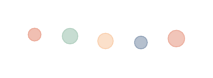
\begin{tikzpicture}
      \foreach \i in {1,...,5}{
        \pgfmathsetmacro{\colorselect}{mod(\i,4)} % Cycle through 4 colors
        \ifcase\colorselect
          \definecolor{dotcolor}{named}{primaryAccent}
        \or
          \definecolor{dotcolor}{named}{secondaryAccent}
        \or
          \definecolor{dotcolor}{named}{tertiaryAccent}
        \or
          \definecolor{dotcolor}{named}{quaternaryAccent}
        \fi
        % Calculate y-position based on a sine wave for a subtle dynamic effect
        \pgfmathsetmacro{\ypos}{sin(\i*72)*1.5} % Adjust multiplier for wave amplitude
        % Vary size slightly based on position in wave or keep constant
        \pgfmathsetmacro{\dotsize}{2.0 + abs(cos(\i*72))*1.0} % Size varies subtly (2.0pt to 3.0pt)
        % Adjust opacity, maybe make it less linear or add slight randomness
        \pgfmathsetmacro{\opacity}{0.4 + 0.3*rand} % Random opacity for texture
        \filldraw[dotcolor!70!white, opacity=\opacity] (\i*0.45-1.35, \ypos pt) circle (\dotsize pt); % Slightly increased spacing
      }
    \end{tikzpicture}
  \end{center}
  % Closing paragraph
  I would welcome the opportunity to discuss how my skills and experience would benefit your organization. Thank you for considering my application. I look forward to hearing from you.
}
\closing{Sincerely,}


% Main document structure
\begin{document}


% This makes @ commands available throughout the document

% Header with personal info
\begin{minipage}[t]{0.6\textwidth}
  \vspace{0.5cm}
  {\Large\textbf{\textcolor{primaryAccent}{\@cvname}}}\\ % Use Cool Blue
  {\small\@cvjobtitle}
\end{minipage}
\begin{minipage}[t]{0.4\textwidth}
  \vspace{0.5cm}
  \raggedright
  {\footnotesize\@cvcontact}
\end{minipage}

\raggedbottom


% Decorative element
\begin{center}
  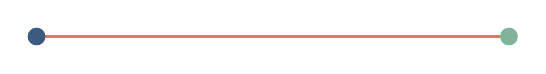
\begin{tikzpicture}
    \draw[secondaryAccent, line width=0.8pt] (0,0) -- (6,0); % Terracotta line
    \filldraw[primaryAccent] (0,0) circle (3pt); % Cool Blue dot
    \filldraw[tertiaryAccent] (6,0) circle (3pt); % Sage Green dot
  \end{tikzpicture}
\end{center}

% Current date
% Replace the current date with this more elegant formatting
\begin{flushright}
  \textit{\today}
\end{flushright}
\vspace{0.8cm}

% Recipient details
\@recipient
\vspace{1.0cm}
\@letterbody
\vspace{1.5cm}

\@closing

\@cvname

\vfill
\begin{center}
  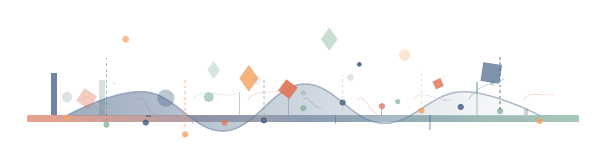
\begin{tikzpicture}
    % Artistic gradient base with new palette
    \shade[left color=secondaryAccent!70, right color=tertiaryAccent!70,
           middle color=primaryAccent!60] % Terracotta, Sage, Cool Blue tints
      (-3.5,0) -- (3.5,0) -- (3.5,-0.08) -- (-3.5,-0.08) -- cycle; % Slightly wider, thinner base

    % Dynamic geometric elements with new colors
    \foreach \i in {-3.2,-2.6,...,3.2} {
      \pgfmathsetmacro{\height}{0.15+0.4*rand}
      \pgfmathsetmacro{\width}{0.03+0.05*rand}
      \pgfmathsetmacro{\colorselect}{mod(round(abs(\i)*10),4)}
      \ifcase\colorselect
        \definecolor{elemcolor}{named}{primaryAccent}
      \or
        \definecolor{elemcolor}{named}{secondaryAccent}
      \or
        \definecolor{elemcolor}{named}{tertiaryAccent}
      \or
        \definecolor{elemcolor}{named}{quaternaryAccent}
      \fi
      \fill[elemcolor, opacity=0.6+0.3*rand] (\i,0) rectangle +(\width,\height); % Slightly less opaque
    }

    % Decorative circles with new colors
    \foreach \i in {-3.0,-2.4,...,3.0} {
      \pgfmathsetmacro{\size}{0.05+0.07*rand}
      \pgfmathsetmacro{\ypos}{0.3+0.2*rand} % Slightly lower position variation
      \pgfmathsetmacro{\colorselect}{mod(round(abs(\i)*10)+1,4)} % Offset color cycle
      \ifcase\colorselect
        \definecolor{circcolor}{named}{quaternaryAccent}
      \or
        \definecolor{circcolor}{named}{tertiaryAccent}
      \or
        \definecolor{circcolor}{named}{secondaryAccent}
      \or
        \definecolor{circcolor}{named}{primaryAccent}
      \fi
      \fill[circcolor!80, opacity=0.5+0.4*rand] (\i,\ypos) circle (\size cm); % Slightly less opaque
    }

    \draw[line width=0.5pt,
          color=primaryAccent!80, opacity=0.5, 
          shading=axis,
          left color=primaryAccent,
          right color=white]
          % Draw a smooth curve with tension
          plot[smooth, tension=0.7] 
          coordinates {(-3,0) (-2,0.3) (-1,-0.2) (0,0.4) (1,-0.1) (2,0.3) (3,0)};
    % Shadow effect removed to fix parsing error
    
    


    % Add dynamic floating shapes with varying sizes and colors
    \foreach \i in {-2.7,-2.2,...,2.7} {
      % Randomize shape position with controlled variation
      \pgfmathsetmacro{\xshift}{0.1*rand}
      \pgfmathsetmacro{\yshift}{0.4*rand}
      \pgfmathsetmacro{\ypos}{0.6+\yshift}
      
      % Select color based on position
      \pgfmathsetmacro{\colorselect}{mod(round(abs(\i*5)),4)}
      \ifcase\colorselect
        \definecolor{elemcolor}{named}{primaryAccent}
      \or
        \definecolor{elemcolor}{named}{secondaryAccent}
      \or
        \definecolor{elemcolor}{named}{tertiaryAccent}
      \or
        \definecolor{elemcolor}{named}{quaternaryAccent}
      \fi
      
      % Randomize shape selection (circles, squares, diamonds)
      \pgfmathsetmacro{\shapetype}{mod(round(abs(\i*7)),3)}
      \pgfmathsetmacro{\size}{0.07+0.06*rand}
      \pgfmathsetmacro{\opacity}{0.6+0.4*rand}
      
      \ifcase\shapetype
        % Circle
        \fill[elemcolor, opacity=\opacity] (\i+\xshift,\ypos) circle (\size cm);
      \or
        % Square with rotation
        \pgfmathsetmacro{\rotation}{45*rand}
        \fill[elemcolor, opacity=\opacity, rotate around={\rotation:(\i+\xshift,\ypos)}] 
          (\i+\xshift-\size,\ypos-\size) rectangle (\i+\xshift+\size,\ypos+\size);
      \or
        % Diamond
        \fill[elemcolor, opacity=\opacity] 
          (\i+\xshift,\ypos+1.4*\size) -- (\i+\xshift+\size,\ypos) -- 
          (\i+\xshift,\ypos-1.4*\size) -- (\i+\xshift-\size,\ypos) -- cycle;
      \fi
    }
    
    % Add subtle accent dots along curve
    \foreach \i in {-3,-2.5,...,3} {
      \pgfmathsetmacro{\ypos}{0.15*sin(\i*60)+0.1*rand}
      \pgfmathsetmacro{\colorselect}{mod(round(abs(\i*3)+2),4)}
      \ifcase\colorselect
        \definecolor{dotcolor}{named}{primaryAccent}
      \or
        \definecolor{dotcolor}{named}{secondaryAccent}
      \or
        \definecolor{dotcolor}{named}{tertiaryAccent}
      \or
        \definecolor{dotcolor}{named}{quaternaryAccent}
      \fi
      \fill[dotcolor, opacity=0.8] (\i, \ypos) circle (0.04cm);
    }
    
    % Add vertical connection lines between some shapes and dots
    \foreach \i in {-2.5,-1.5,...,2.5} {
      \pgfmathsetmacro{\colorselect}{mod(round(abs(\i)+1),4)}
      \ifcase\colorselect
        \definecolor{linecolor}{named}{primaryAccent}
      \or
        \definecolor{linecolor}{named}{secondaryAccent}
      \or
        \definecolor{linecolor}{named}{tertiaryAccent}
      \or
        \definecolor{linecolor}{named}{quaternaryAccent}
      \fi
      \pgfmathsetmacro{\ystart}{0.15*sin(\i*60)}
      \pgfmathsetmacro{\yend}{0.5+0.3*rand}
      \draw[linecolor, opacity=0.4, line width=0.5pt, dash pattern=on 1pt off 1pt] 
        (\i,\ystart) -- (\i,\yend);
    }

    % Dynamic connecting lines with new colors
    \foreach \i in {-2.8,-2.1,...,2.8} {
      \pgfmathsetmacro{\nextx}{\i+0.4+0.2*rand}
      \pgfmathsetmacro{\nexty}{0.25+0.3*rand}
      \pgfmathsetmacro{\colorselect}{mod(round(abs(\i)*10),3)} % Cycle through first 3 accents
      \ifcase\colorselect
        \definecolor{linecolor}{named}{primaryAccent}
      \or
        \definecolor{linecolor}{named}{secondaryAccent}
      \or
        \definecolor{linecolor}{named}{tertiaryAccent}
      \fi
      \draw[linecolor!60, opacity=0.5, line width=0.25pt] % Thinner, less opaque lines
        (\i,0.2) to[out=60, in=200] (\nextx,\nexty);
    }

    % Accent dots with new colors
    \foreach \i in {-2.5,-1.5,...,2.5} { % Adjusted positions
      \pgfmathsetmacro{\colorselect}{mod(round(abs(\i)+2),4)}
      \ifcase\colorselect
        \definecolor{dotcolor}{named}{primaryAccent}
      \or
        \definecolor{dotcolor}{named}{secondaryAccent}
      \or
        \definecolor{dotcolor}{named}{tertiaryAccent}
      \or
        \definecolor{dotcolor}{named}{quaternaryAccent}
      \fi
      \fill[dotcolor, opacity=0.8] (\i, -0.04) circle (0.06pt); % Smaller dots on the base line
    }
  \end{tikzpicture}
\end{center}
\makeatother
\end{document}
